\subsection{Zariski 环的完备化}

命题 9。设 A 为交换 Noether 环，m 为 A 的理想；赋予 A m-进拓扑。要使 \(\hat{\mathbf{A}}\) 成为忠实平坦的 A-模，充要条件是 A 为 Zariski 环。

对于每个有限生成的 A-模 M，典范映射 \(M \to M \otimes_{A} \hat{A}\) 可识别为从 M 到其关于 m-进拓扑的 Hausdorff 完备化的典范映射 \(M \to \hat{M}\)（第 4 号，定理 3），而该映射的核就是 M 中关于此拓扑的 \(\{0\}\) 的闭包。由于我们已经知道 \(\hat{A}\) 是平坦的 A-模（第 4 号，定理 3），命题由忠实平坦模的刻画（第一章，第 3 节，第 1 号，命题 1（b））和 Zariski 环的刻画（第 3 号，命题 6）得出。

若 A 是 Zariski 环且 E 是有限生成的 A-模，则根据命题 9，我们可以将 E 识别为 \(\hat{E}\) 的子集，借助典范映射 \(j_{E}: E \to \hat{E}\)。在此识别下：

推论 1。设 A 为 Zariski 环，E 为有限生成的 A-模，F 为 E 的子模。则 \(\mathbf{F} = \hat{\mathbf{F}} \cap \mathbf{E} = (\hat{\mathbf{A}}\mathbf{F}) \cap \mathbf{E}\)。

这是第一章第 3 节第 5 号命题 10（ii）的特殊情形，也可由第 3 号命题 6 得出。

推论 2。设 A 为 Zariski 环，E 为有限生成的 A-模。若 \(\hat{\mathbf{E}}\) 是自由的 \(\hat{\mathbf{A}}\)-模，则 E 是自由的 A-模。

设 \(\mathfrak{m}\) 为 \(\mathbf{A}\) 的定义理想，因而包含于 \(\mathbf{A}\) 的 Jacobson 根中。我们应用第二章第 3 节第 5 号命题 5 的判别法：典范映射 \(j_{\mathrm{E}}: \mathrm{E} \to \hat{\mathrm{E}}\) 定义了双射 \(i_{\mathrm{E}}: \mathrm{E} / \mathfrak{m}\mathrm{E} \to \hat{\mathrm{E}} / (\mathfrak{m}\mathrm{E})^{\wedge}\)；同样，典范映射 \(j_{\mathrm{A}}: \mathrm{A} \to \hat{\mathrm{A}}\) 定义了双射 \(i_{\mathrm{A}}: \mathrm{A} / \mathfrak{m} \to \hat{\mathrm{A}} / \hat{\mathfrak{m}}\)，它是环同构。于是 \((\mathfrak{m}\mathrm{E})^{\wedge} = \hat{\mathrm{A}}. \mathfrak{m}\mathrm{E} = \hat{\mathfrak{m}}\hat{\mathrm{E}}\)（第 4 号，定理 3），所以 \(\hat{\mathrm{E}} / (\mathfrak{m}\mathrm{E})^{\wedge}\) 具有一个 \((\hat{\mathrm{A}} / \hat{\mathfrak{m}})\)-模结构，并且（借助 \(i_{\mathrm{A}}\)）具有一个 \((\mathrm{A} / \mathfrak{m})\)-模结构。立即可见，\(i_{\mathrm{E}}\) 是 \((\mathrm{A} / \mathfrak{m})\)-线性的，因而是一个 \((\mathrm{A} / \mathfrak{m})\)-模同构。由于 \(\hat{\mathrm{E}} / \hat{\mathfrak{m}}\hat{\mathrm{E}}\) 是自由的 \((\hat{\mathrm{A}} / \hat{\mathfrak{m}})\)-模，\(\mathrm{E} / \mathfrak{m}\mathrm{E}\) 是自由的 \((\mathrm{A} / \mathfrak{m})\)-模。

另一方面，令 \(v: \mathfrak{m} \otimes_{\mathbf{A}} \mathbf{E} \to \mathbf{E}\) 为典范同态；由于 \((\mathfrak{m} \otimes_{\mathbf{A}} \mathbf{E}) \otimes_{\mathbf{A}} \hat{\mathbf{A}}\) 典范地识别为 \(\hat{\mathfrak{m}} \otimes_{\mathbf{A}} \hat{\mathbf{E}}\)，而 \(\mathbf{E} \otimes_{\mathbf{A}} \hat{\mathbf{A}}\) 识别为 \(\hat{\mathbf{E}}\)（第 4 号，定理 3），\(\hat{\mathbf{E}}\) 是自由的 \(\hat{\mathbf{A}}\)-模这一假设蕴含同态 \(v \otimes 1: \hat{\mathfrak{m}} \otimes_{\hat{\mathbf{A}}} \hat{\mathbf{E}} \to \hat{\mathbf{E}}\) 是单射。由于 \(\hat{\mathbf{A}}\) 是忠实平坦的 A-模（命题 9），我们得到 \(v\) 是单射（第一章，第 3 节，第 1 号，命题 2），因而上述判别法的应用条件确已满足。

推论 3。设 A 为 Zariski 环，且 \(\hat{\mathbf{A}}\) 是整环，\(\mathfrak{a}\) 是 A 的理想。若理想 \(\mathfrak{a}\hat{\mathbf{A}}\) 在 \(\hat{\mathbf{A}}\) 中是主理想，则 \(\mathfrak{a}\) 是主理想。这是推论 2 的特殊情形。

推论 4。设 A 为 Zariski 环，且 \(\hat{\mathbf{A}}\) 是整环，L 为 \(\hat{\mathbf{A}}\) 的分式域，\(\mathbf{K} \subset \mathbf{L}\) 为 A 的分式域；则 \(\hat{\mathbf{A}} \cap \mathbf{K} = \mathbf{A}\)。

显然 \(\mathbf{A} \subset \hat{\mathbf{A}} \cap \mathbf{K}\)；另一方面，若 \(x \in \hat{\mathbf{A}} \cap \mathbf{K}\)，则 \(\hat{\mathbf{A}}x \subset \hat{\mathbf{A}}\)，因而由于 \(\hat{\mathbf{A}}x = \hat{\mathbf{A}} \otimes_{\mathbf{A}} (\mathbf{A}x)\)（第 4 号，定理 3），有 \(\hat{\mathbf{A}} \otimes_{\mathbf{A}} ((\mathbf{A}x + \mathbf{A}) / \mathbf{A}) = 0\)。由于 \(\hat{\mathbf{A}}\) 是忠实平坦的 A-模（命题 9），我们得到 \(\mathbf{A}x \subset \mathbf{A}\)，所以 \(x \in \mathbf{A}\)。

推论 5。设 A 为交换 Noether 环，E、F 为两个有限生成的 A-模，u: E → F 为 A-同态。对于 A 的每个极大理想 m，令 A(m)（分别为 E(m)、F(m)）表示 A（分别为 E、F）关于 m-进拓扑的 Hausdorff 完备化，令 u(m): E(m) → F(m) 为 u 所对应的同态。u 为单射（分别为满射、双射、零映射）的充要条件是：对于 A 的每个极大理想 m，u(m) 都具有相应性质。

我们知道，要使 \(u\) 为单射（分别为满射、双射、零映射），充要条件是 \(u_{\mathfrak{m}}: \mathrm{E}_{\mathfrak{m}} \to \mathrm{F}_{\mathfrak{m}}\) 对每个极大理想 \(\mathfrak{m}\)（属于 \(\mathbf{A}\)）都具有相应性质（第二章，第 3 节，第 3 号，定理 1）。现在注意到，\(\mathbf{A}_{\mathfrak{m}}\) 是 Noether 局部环（第二章，第 2 节，第 4 号，命题 10 的推论 2），因而是 Zariski 环，并且存在典范的 A-代数同构 \(\hat{\mathbf{A}}_{\mathfrak{m}} \to \mathbf{A}(\mathfrak{m})\)（第 2 节，第 13 号，命题 18）。另一方面（第 4 号开头），存在交换图

\[
\begin{array}{l} \mathrm{E} _ {\mathfrak {m}} \otimes_ {\mathbf {A} _ {\mathfrak {m}}} \mathrm{A} (\mathfrak {m}) \longrightarrow \mathrm{E} \otimes_ {\mathbf {A}} \mathrm{A} (\mathfrak {m}) \longrightarrow \mathrm{E} (\mathfrak {m}) \\ u _ {\mathfrak {m}} \otimes 1 \Biggl \downarrow \qquad \qquad \qquad \qquad \Biggl \downarrow u \otimes 1 \qquad \qquad \Biggl \downarrow u (\mathfrak {m}) \\ \mathrm{F} _ {\mathfrak {m}} \otimes_ {\mathbf {A} _ {\mathfrak {m}}} \mathrm{A} (\mathfrak {m}) \longrightarrow \mathrm{F} \otimes_ {\mathbf {A}} \mathrm{A} (\mathfrak {m}) \longrightarrow \mathrm{F} (\mathfrak {m}) \end{array}
\]

左侧的水平箭头来自张量积的结合律以及同构 \(E_{m} \rightarrow E \otimes_{A} A_{m}\)、\(F_{m} \rightarrow F \otimes_{A} A_{m}\)；由于 E、F 是有限生成的 A-模，由第 4 号定理 3 可知该图的各行都是同构。因此问题归结为证明：\(u_{m}\) 是单射（分别为满射、双射、零映射）当且仅当 \(u_{m} \otimes 1\) 具有相应性质。但这是命题 9 所说的 \(\hat{A}_{m}\)（因而 \(A(m)\) 也）是忠实平坦的 \(A_{m}\)-模这一事实的结果（第一章，第 3 节，第 1 号，命题 1 和 2）。

命题 10。设 A、B 为两个 Zariski 环，\(\hat{A}\)、\(\hat{B}\) 为它们的完备化，\(f\colon A\to B\) 为连续环同态，\(\hat{f}\colon\hat{A}\to\hat{B}\) 为由 \(f\) 取完备化得到的同态；若 \(\hat{f}\) 是双射，则 B 是忠实平坦的 A-模。

由于 A、B 是 Hausdorff 的，\(\hat{f}\) 为双射这一假设首先蕴含 \(f\) 是单射。将 A（代数地）识别为 \(f(A)\)，这是借助 \(f\) 完成的；随后将 \(\hat{A}\) 识别为 \(\hat{B}\)，所对应的映射为 \(\hat{f}\)，于是得到包含关系 \(A \subset B \subset \hat{A} = \hat{B}\)；我们知道 \(\hat{A}\) 既是忠实平坦的 A-模，也是忠实平坦的 B-模（命题 9）；由此得到 B 是忠实平坦的 A-模（第一章，第 3 节，第 4 号，注 2）。

命题 11。设 A 为 Noether 局部环，m 为其极大理想，\(\hat{\mathbf{A}}\) 为其 m-进完备化，B 为满足 \(\mathbf{A} \subset \mathbf{B} \subset \hat{\mathbf{A}}\) 的环。假设 B 是 Noether 局部环，其极大理想 n 满足关系 \(n = mB\)。则

\[
\mathfrak {n} ^ {k} = \mathfrak {m} ^ {k} \mathrm{B} = \hat {\mathfrak {m}} ^ {k} \cap \mathrm{B}
\]

对所有 \(k \geqslant 1\)，\(\mathfrak{n}\)-进拓扑在 \(\mathbf{B}\) 上由 \(\hat{\mathfrak{m}}\)-进拓扑在 \(\hat{\mathbf{A}}\) 上诱导，\(\mathbf{B}\) 是忠实平坦的 \(\mathbf{A}\)-模，并且存在从 \(\hat{\mathbf{A}}\) 到 \(\mathfrak{n}\)-进完备化 \(\hat{\mathbf{B}}\) 的 \(\mathbf{B}\) 的同构，它延拓 \(\mathbf{A} \to \mathbf{B}\) 的典范单射。

只需验证关系 \(n^{k} = \hat{m}^{k} \cap B\)，因为 B 在 \(\hat{A}\) 中稠密，且 n-进拓扑由 \(\hat{m}\)-进拓扑诱导，所以最后一个断言由一般拓扑学第二章第 3 节第 9 号命题 18 的推论 1 得出，倒数第二个断言由命题 10 得出。单射 \(j_{A}: A \to \hat{A}\)（分别为 \(j_{B}: B \to \hat{A}\)）取商后定义了一个单同态

\[
i _ {\mathbf {A}} \colon \mathrm{A} / (\hat {\mathfrak {m}} \cap \mathrm{A}) \rightarrow \hat {\mathrm{A}} / \hat {\mathfrak {m}}
\]

（分别地，\(i_{B}\)：B/(m ∩ B) → Â/m）。我们知道 m ∩ A = m 且 \(i_{A}\) 是双射，因而 \(i_{B}\) 也是双射；这表明 B/(m ∩ B) 是域，所以 m ∩ B 是 B 的极大理想，从而 m ∩ B = n。~由于 \(\hat{A} = A + \hat{m}\)，\(B = A + n = A + mB\)；由 k 归纳可得

\[
\mathbf {B} = \mathbf {A} + \mathfrak {m} ^ {k} \mathbf {B} = \mathbf {A} + \mathfrak {n} ^ {k}
\]

对所有 \(k > 1\) 都成立。由于 \(\mathfrak{n}^k \subset \hat{\mathfrak{m}}^k \cap \mathbf{B}\)，只需证明 \(\hat{\mathfrak{m}}^k \cap \mathbf{B} \subset \mathfrak{n}^k\)；若 \(b \in \hat{\mathfrak{m}}^k \cap \mathbf{B}\)，可写成 \(b = a + z\)，其中 \(a \in \mathbf{A}\)、\(z \in \mathfrak{n}^k\)；于是

\[
a = b - z \in \hat {\mathfrak {m}} ^ {k} \cap \mathrm{A} = \mathfrak {m} ^ {k} \subset \mathfrak {n} ^ {k}
\]

且 \(b \in \mathfrak{n}^k\)。

* 此结果的一个重要应用情形如下：B 是完备赋值域上 n 个变量的整幂级数环，它们在 0 的邻域内收敛；A 是局部环

\[
\mathrm{K} [ \mathrm{X} _ {1}, \dots , \mathrm{X} _ {n} ] _ {\mathfrak {p}}
\]

其中 p 是由不含常数项的多项式组成的极大理想，\(\hat{A}\) 是形式幂级数环 \(K[[X_{1},\ldots,X_{n}]]\)。*

\pandocbounded{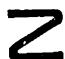
\includegraphics[keepaspectratio]{images/part002_72a4a9a7.jpg}}

注。满足 \(A \subset B \subset \hat{A}\)、其极大理想 n 等于 mB 且其 n-进拓扑由 \(\hat{A}\) 上的 m-进拓扑诱导的局部环 B 不一定是 Noether 环（习题 14）。

命题 12。设 A 为交换 Noether 环，m 为 A 的理想，S 为 A 的乘性子集 \(1 + m\)，E 为有限生成的 A-模。在这些条件下：

\begin{enumerate}
\def\labelenumi{(\roman{enumi})}
\item
  \(\mathbf{S}^{-1}\mathbf{A}\) 是 Zariski 环，且其拓扑为 \((\mathbf{S}^{-1}\mathfrak{m})\)-进拓扑。
\item
  典范映射 \(f \colon \mathbf{E} \to \mathbf{S}^{-1}\mathbf{E}\) 在 \(\mathbf{E}\) 赋予 \(\mathfrak{m}\)-进拓扑、\(\mathbf{S}^{-1}\mathbf{E}\) 赋予 \((\mathbf{S}^{-1}\mathfrak{m})\)-进拓扑时连续，且 \(\hat{f} \colon \hat{\mathbf{E}} \to (\mathbf{S}^{-1}\mathbf{E})^{\wedge}\) 是同构。
\end{enumerate}

\(1 + (\mathbf{S}^{-1}\mathfrak{m})\) 中的每个元素都具有如下形式：

\[
1 + (m / \left(1 + m ^ {\prime}\right)) = (1 + m + m ^ {\prime}) / (1 + m)
\]

其中 \(m \in m\) 且 \(m' \in m\)；所以它在 \(S^{-1}A\) 中可逆，这证明 \(S^{-1}m\) 包含于 \(S^{-1}A\) 的 Jacobson 根；由于 \(S^{-1}A\) 是 Noether 环（第二章，第 2 节，第 4 号，命题 10 的推论 2），\(S^{-1}A\) 连同 \((\mathrm{S}^{-1}\mathrm{m})\)-进拓扑是 Zariski 环，这证明了 (i)。证明 (ii)。对于所有 n \textgreater{} 0，

\[
\bar {f} ^ {- 1} ((S ^ {- 1} m) ^ {n} E) = \bar {f} ^ {- 1} (S ^ {- 1} (m ^ {n} E)) = m ^ {n} E:
\]

显然首先 \(f(\mathfrak{m}^n\mathrm{E}) \subset \mathrm{S}^{-1}\mathfrak{m}^n\mathrm{E}\)；反之，设 \(x\) 是 \(f^{-1}(\mathrm{S}^{-1}\mathfrak{m}^n\mathrm{E})\) 的一个元素；则存在 \(m', m''\) 属于 \(\mathfrak{m}\) 的元素以及 \(x'' \in \mathfrak{m}^n\mathrm{E}\)，使得 \((1 + m')((1 + m'')x - x'') = 0\)，从而 \((1 - m)x = x'\)，其中

\[
m = - \left(m ^ {\prime} + m ^ {\prime \prime} + m ^ {\prime} m ^ {\prime \prime}\right) \in \mathfrak {m}
\]

且 \(x' = (1 + m')x'' \in \mathfrak{m}^n\mathrm{E}\)；我们得到

\[
x = (1 + m + \dots + m ^ {n - 1}) x ^ {\prime} + m ^ {n} x \in \mathfrak {m} ^ {n} \mathrm{E}.
\]

这就证明了 \(f\) 是严格态射。此外，\(f\) 的核，即所有 \(x \in \mathbf{E}\) 满足存在某个 \(s \in \mathbf{S}\) 使得 \(sx = 0\) 的集合，与典范映射 \(j: \mathbf{E} \to \hat{\mathbf{E}}\) 的核相同（第 2 号，命题 5）。于是存在拓扑同构 \(f_0: j(\mathbf{E}) \to f(\mathbf{E})\)，使得 \(f = f_0 \circ j\)；由于 \(j\) 是拓扑同构，问题归结为验证 \(f(\mathbf{E})\) 在 \(\mathbf{S}^{-1}\mathbf{E}\) 中稠密。现在 \(\mathbf{S}^{-1}\mathbf{E}\) 的每个元素都可写成 \(x / (1 - m)\)，其中 \(m \in \mathfrak{m}\)，并且立即可验证

\[
x / (1 - m) \equiv ((1 + m + \dots + m ^ {n - 1}) x) / 1 (\mathrm{mod.} \mathrm{S} ^ {- 1} \mathrm{m} ^ {n} \mathrm{E})
\]

这就完成了证明。

